\documentclass[../main.tex]{subfiles}

\begin{document}

\subsection{En mycket viktig teknik vid programkonstruktion är "stegvis förfining".
Förklara denna teknik med hjälp av ett exempel. (OBS! inte källkod).}

\textbf{Exempel: Morgonrutin.}
\\
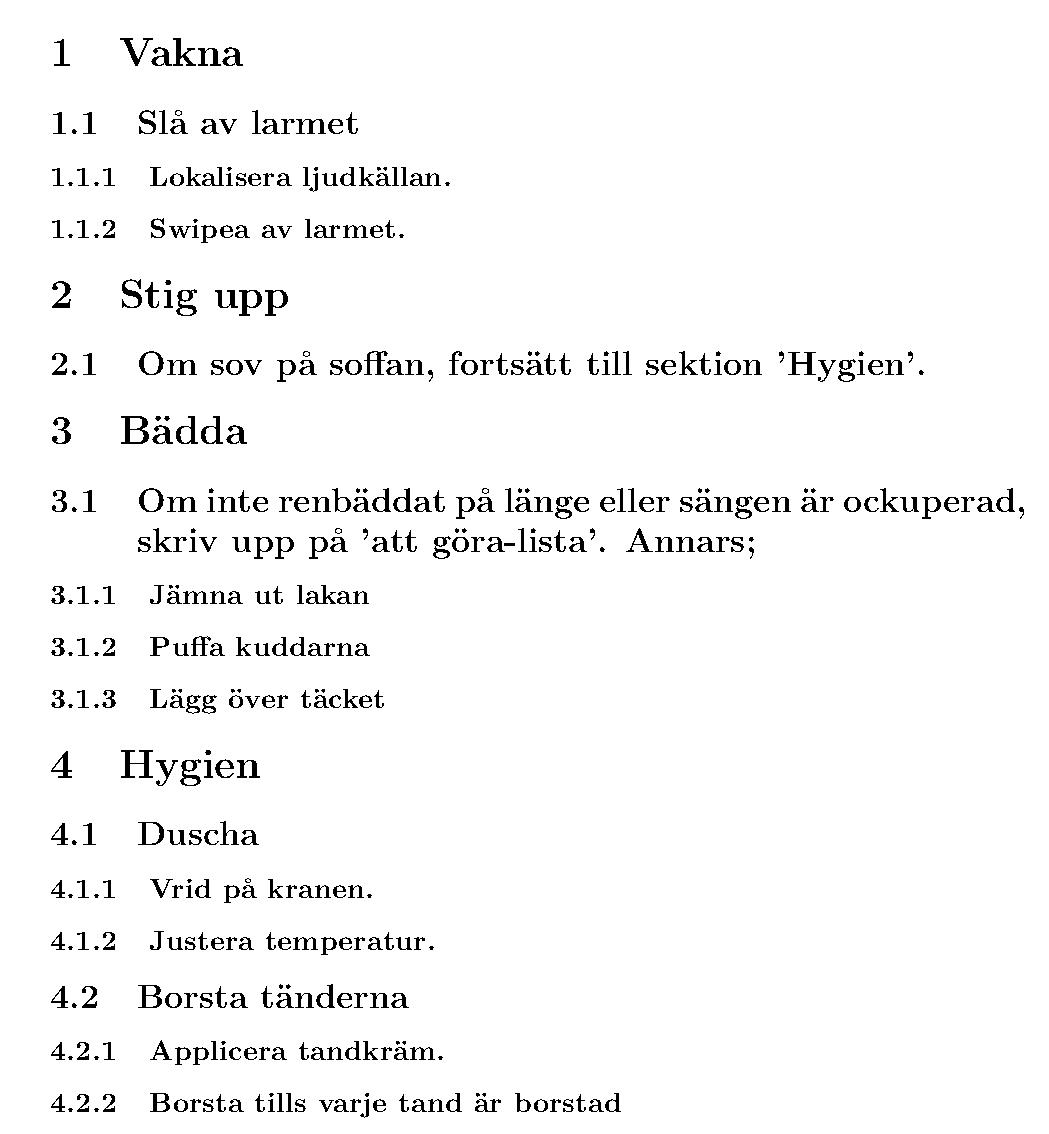
\includegraphics[width=10cm, height=12cm]{sec1/Figs/stegvis.png}

\newpage

\end{document}

